\documentclass[border=8pt]{standalone}
\usepackage{fontspec}
\setmainfont{Carlito}
\setsansfont{Carlito}
\usepackage{xcolor}
\usepackage{tikz}
\usetikzlibrary{positioning, arrows.meta, calc, backgrounds, shapes.geometric, fit}

\definecolor{canvabg}{RGB}{246,244,241}
\pagecolor{canvabg}

\definecolor{flowblue}{RGB}{70,130,180}
\definecolor{lostred}{RGB}{200,90,80}
\definecolor{solutionteal}{RGB}{50,140,140}
\definecolor{regamber}{RGB}{200,150,50}
\definecolor{neutralgrey}{RGB}{100,100,110}
\definecolor{linegrey}{RGB}{200,195,188}

\pgfdeclarelayer{boundary}
\pgfsetlayers{background,boundary,main}

\begin{document}
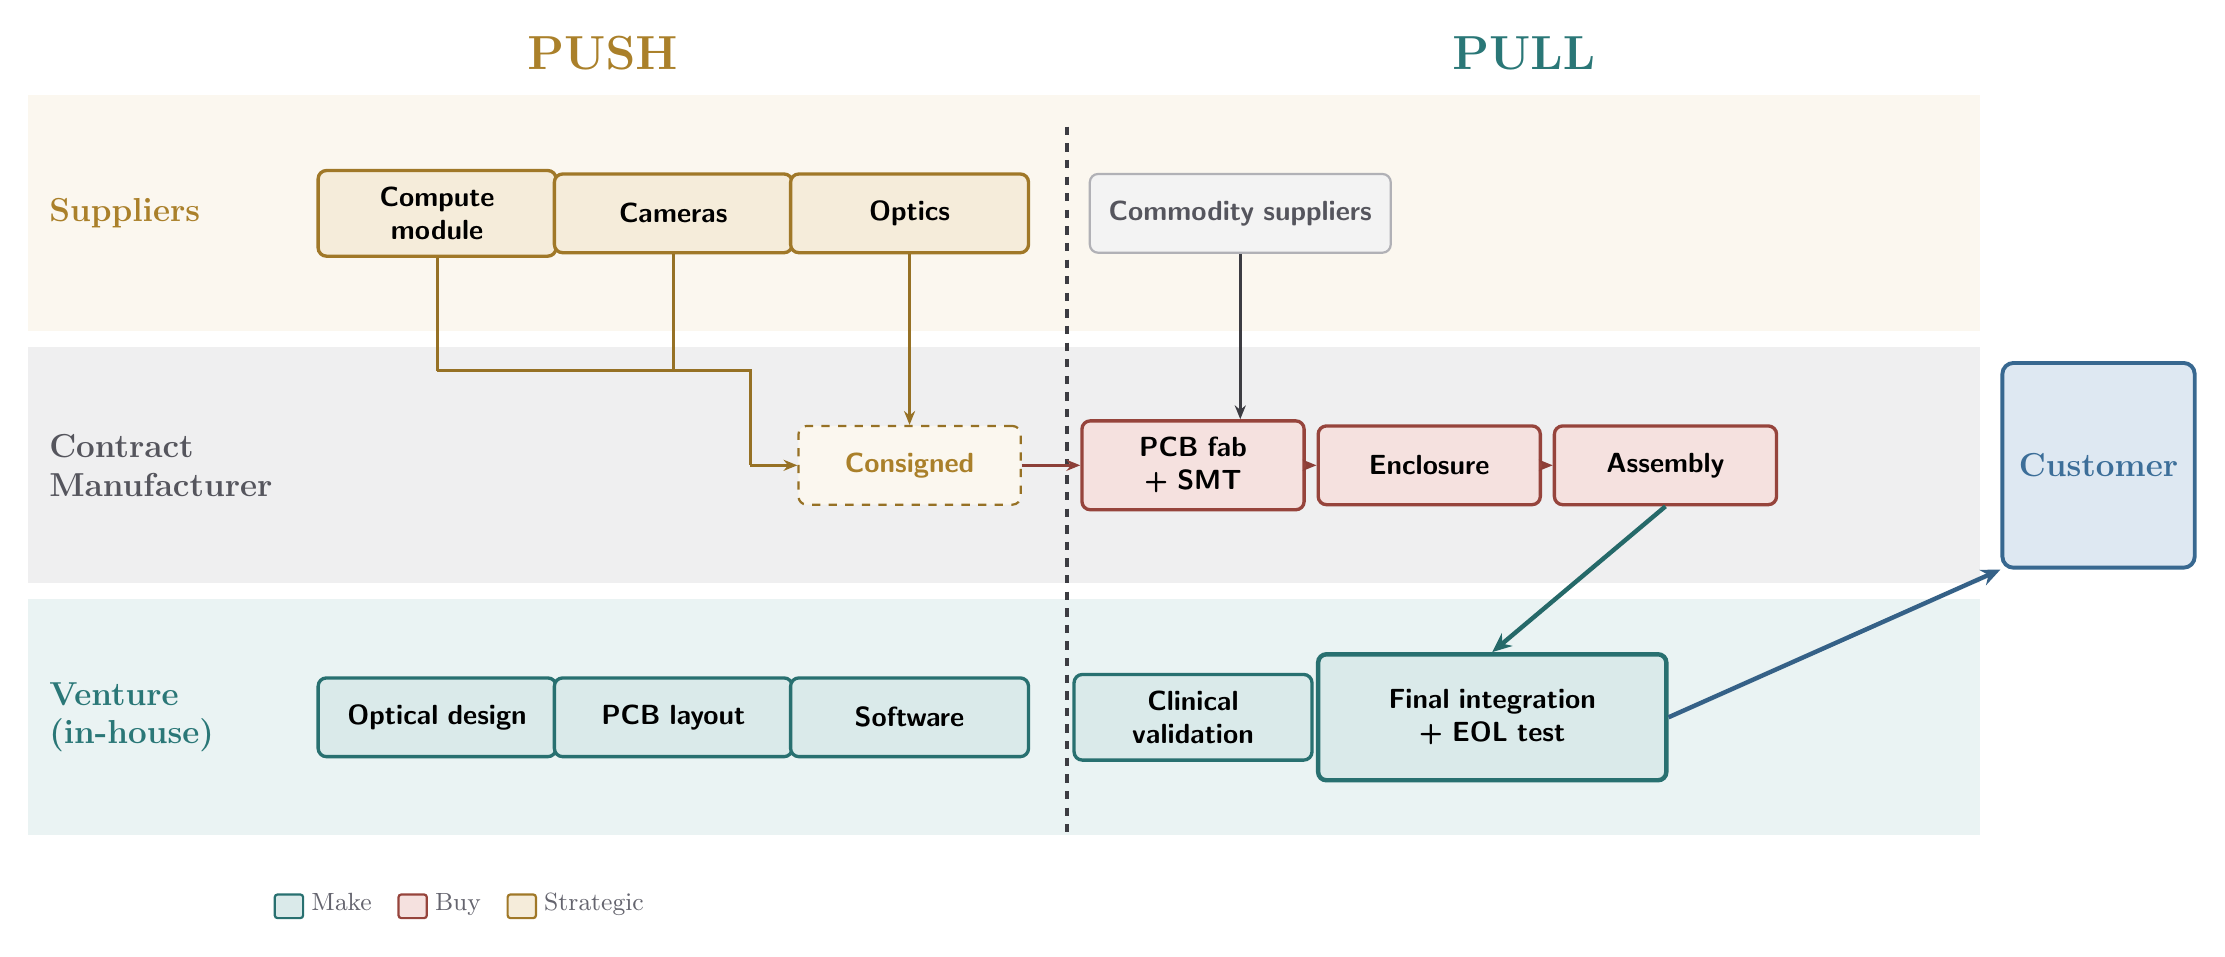
\begin{tikzpicture}[
    every node/.style={font=\sffamily},
    strat node/.style={rectangle, rounded corners=3pt, line width=1.2pt,
                       draw=regamber!80!black, fill=regamber!18,
                       align=center, inner sep=6pt, text width=2.6cm,
                       minimum height=1.0cm},
    buy node/.style={rectangle, rounded corners=3pt, line width=1.2pt,
                     draw=lostred!75!black, fill=lostred!18,
                     align=center, inner sep=6pt, text width=2.4cm,
                     minimum height=1.0cm},
    make node/.style={rectangle, rounded corners=3pt, line width=1.2pt,
                      draw=solutionteal!80!black, fill=solutionteal!18,
                      align=center, inner sep=6pt, text width=2.6cm,
                      minimum height=1.0cm},
    cust node/.style={rectangle, rounded corners=4pt, line width=1.4pt,
                      draw=flowblue!80!black, fill=flowblue!18,
                      align=center, inner sep=6pt},
    arr/.style={-{Stealth[length=5pt,width=4pt]}, line width=1.0pt},
    bigarr/.style={-{Stealth[length=7pt,width=6pt]}, line width=1.6pt},
  ]

  % ========= LANE BACKGROUNDS =========
  \begin{pgfonlayer}{background}
    \fill[regamber!8]      (-2.8, -0.2) rectangle (22, -3.2);
    \fill[neutralgrey!10]  (-2.8, -3.4) rectangle (22, -6.4);
    \fill[solutionteal!10] (-2.8, -6.6) rectangle (22, -9.6);
  \end{pgfonlayer}

  % ========= LANE LABELS =========
  \node[anchor=west, font=\large\bfseries, text=regamber!85!black]
    at (-2.65, -1.7) {Suppliers};
  \node[anchor=west, font=\large\bfseries, text=neutralgrey!85!black,
        align=left, text width=2.6cm]
    at (-2.65, -4.9) {Contract\\Manufacturer};
  \node[anchor=west, font=\large\bfseries, text=solutionteal!85!black,
        align=left, text width=2.6cm]
    at (-2.65, -8.1) {Venture\\(in-house)};

  % ========= PUSH/PULL BOUNDARY (on dedicated layer) =========
  \begin{pgfonlayer}{boundary}
    \draw[neutralgrey!60!black, dashed, line width=1.2pt]
      (10.4, -0.6) -- (10.4, -9.6);
  \end{pgfonlayer}

  % BIG push/pull labels
  \node[anchor=south, font=\LARGE\bfseries, text=regamber!85!black]
    at (4.5, 0.0) {PUSH};
  \node[anchor=south, font=\LARGE\bfseries, text=solutionteal!85!black]
    at (16.2, 0.0) {PULL};

  % ========= SUPPLIERS LANE =========
  \node[strat node] (cm)  at (2.4, -1.7) {\bfseries Compute module};
  \node[strat node] (cam) at (5.4, -1.7) {\bfseries Cameras};
  \node[strat node] (opt) at (8.4, -1.7) {\bfseries Optics};

  \node[rectangle, rounded corners=3pt, line width=0.8pt,
        draw=neutralgrey!50, fill=neutralgrey!8,
        align=center, inner sep=6pt, text width=3.4cm,
        minimum height=1.0cm] (commod) at (12.6, -1.7)
    {\color{neutralgrey!85!black}\bfseries Commodity suppliers};

  % ========= CM LANE =========
  \node[rectangle, rounded corners=3pt, line width=0.8pt,
        draw=regamber!75!black, dashed, fill=regamber!8,
        align=center, inner sep=6pt, text width=2.4cm,
        minimum height=1.0cm] (consign) at (8.4, -4.9)
    {\color{regamber!85!black}\bfseries Consigned};

  \node[buy node] (pcb)  at (12.0, -4.9) {\bfseries PCB fab + SMT};
  \node[buy node] (encl) at (15.0, -4.9) {\bfseries Enclosure};
  \node[buy node] (asm)  at (18.0, -4.9) {\bfseries Assembly};

  % ========= VENTURE LANE =========
  \node[make node] (od)   at (2.4, -8.1) {\bfseries Optical design};
  \node[make node] (pcbd) at (5.4, -8.1) {\bfseries PCB layout};
  \node[make node] (sw)   at (8.4, -8.1) {\bfseries Software};
  \node[make node] (cv)   at (12.0, -8.1) {\bfseries Clinical\\validation};
  \node[make node, text width=4.0cm, line width=1.6pt,
        minimum height=1.6cm] (intg) at (15.8, -8.1)
    {\bfseries Final integration\\+ EOL test};

  % ========= CUSTOMER TERMINUS =========
  \node[cust node, minimum width=2.0cm, minimum height=2.6cm,
        font=\large\bfseries\color{flowblue!85!black}]
    (cust) at (23.5, -4.9) {Customer};

  % ========= ARROWS =========
  % 1. Strategic suppliers -> consignment
  % Compute module + Cameras: drop into a high horizontal trunk at y=-3.7,
  % trunk runs right to a point just left of consign, drops down to
  % consign-centre y, then enters consign with a clear horizontal arrow
  % from the LEFT.
  \coordinate (jcm)        at (2.4, -3.7);
  \coordinate (jcam)       at (5.4, -3.7);
  \coordinate (preconsign) at ($(consign.west) + (-0.6,0)$);
  \draw[color=regamber!75!black, line width=1.0pt] (cm.south)  -- (jcm);
  \draw[color=regamber!75!black, line width=1.0pt] (cam.south) -- (jcam);
  \draw[color=regamber!75!black, line width=1.0pt] (jcm) -| (preconsign);
  \draw[arr, color=regamber!75!black] (preconsign) -- (consign.west);
  % Optics: straight down into consign.north
  \draw[arr, color=regamber!75!black] (opt.south) -- (consign.north);

  % 2. Commodity supplier -> CM
  \draw[arr, color=neutralgrey!60!black]
    (commod.south) -- (pcb.north -| commod.south);

  % 3. Intra-CM chain
  \draw[arr, color=lostred!70!black] (consign.east) -- (pcb.west);
  \draw[arr, color=lostred!70!black] (pcb.east)     -- (encl.west);
  \draw[arr, color=lostred!70!black] (encl.east)    -- (asm.west);

  % 4. CM assembly -> Venture final integration (boldest single arrow)
  \draw[bigarr, color=solutionteal!75!black] (asm.south) -- (intg.north);

  % 5. Final integration -> Customer
  \draw[bigarr, color=flowblue!75!black] (intg.east) -- (cust.south west);

  % ========= LEGEND STRIP =========
  \node[anchor=west, font=\small, text=neutralgrey] at (0.2, -10.5) {%
    \tikz[baseline=-0.4ex]{\fill[solutionteal!18, draw=solutionteal!80!black, line width=0.8pt, rounded corners=1pt] (0,-0.15) rectangle (0.36,0.15);}\;Make\quad
    \tikz[baseline=-0.4ex]{\fill[lostred!18, draw=lostred!75!black, line width=0.8pt, rounded corners=1pt] (0,-0.15) rectangle (0.36,0.15);}\;Buy\quad
    \tikz[baseline=-0.4ex]{\fill[regamber!18, draw=regamber!80!black, line width=0.8pt, rounded corners=1pt] (0,-0.15) rectangle (0.36,0.15);}\;Strategic
  };

\end{tikzpicture}
\end{document}
